\documentclass[a4paper,10pt]{article}
\usepackage[utf8]{inputenc}
\usepackage[english]{babel}
\usepackage{geometry}
\usepackage{graphicx}
\usepackage{blindtext}
\usepackage{titling}
\usepackage[nottoc]{tocbibind} %Adds "References" to the table of contents
\usepackage{fontawesome}
\usepackage{url}
\usepackage{hyperref}
\usepackage{float}
\usepackage{subcaption}
\usepackage{color}
\hypersetup{
	colorlinks=true,
	linkcolor=black,
	filecolor=magenta,      
	urlcolor=blue,
}


\newcommand{\github}[2][13pt]{\hspace{5pt}\faGithub\hspace{5pt}\fontsize{#1}{0}\url{#2}}

%Document title, author and date (empty)
\title{Travelling salesman problem}
\author{Giovanni Sorice - 606915}
\date{July 2020}

% Definition of \maketitle
\makeatletter         
\def\@maketitle{
	\raggedright
	%\includegraphics[width = 40mm]{logo.jpg}\\[8ex]
	\begin{center}
		{\Huge \bfseries \sffamily \@title }\\[4ex] 
		{\Large  \@author}\\[4ex] 
		\@date\\[8ex]
		
\includegraphics[scale = 0.35]{logo-Pisa.jpeg}
\end{center}}
\makeatother

%Beginning of the document
\begin{document}
	

		\maketitle
		\begin{abstract}
			The assignment required to implement three different solutions for Travelling salesman problem. I initially developed a \textit{sequential} version, needed as a baseline and performance comparison for further implementations. The parallel versions developed are based on c++ standard thread and on FastFlow framework.
		\end{abstract}

	
	\section{Introduction}
	This report describes the framework developer to execute the traveling salesman problem with genetic algorithm.
	The TSP is a NP-hard problem and for this reason during the year many heuristic and approximation algorithms were invented and used. One of the most successfully category of algorithms for the TSP problem are the genetic algorithms.
	A genetic algorithm works by building a population of chromosomes, usually randomly generated, which is a set of possible solutions to the optimization problem. During each iteration of the algorithm, the population is randomly altered in hopes of creating new chromosomes that have better evaluation scores. The next generation population of chromosomes is randomly selected from the current generation with selection probability based on the evaluation score of each chromosome, adding some randomly changing to the previous population chromosomes. There are several variant of genetic algorithms structure. I choose also to take in account of the best previously population chromosomes for the current population.
	\\
	Usually a genetic algorithm is divided in more phases:
	\begin{itemize}
		\item Initialization;
		\item Evaluation;
		\item Selection;
		\item Reproduction;
		\item Crossover;
		\item Mutation.
	\end{itemize}

	\subsection{Measures}
	We need some measures to understand the real advantages of using a parallel implementation. The common measures used in this case are speedup and scalability.
	\subsubsection{Speedup}
	The speedup is used to compare the time needed to execute a specific task sequentially with the time needed to do the same task in parallel. The ratio among the time spent by the sequential and the time spent by the parallel is called Speedup. We hope that it was linearly proportional to the number of parallel degree used and for this reason the time spent doing the task decrease as 1/k where k is the parallelism degree. Unfortunately, there are more things to keep in mind (overhead) and usually the rate of speedup is not the expected.
	The speedup is computed as follows.
	\begin{equation}
	speedup(n)=\frac{T_{seq}}{T_{par}}
	\end{equation}
	
	\subsubsection{Scalability}
	The scalability is the ration between the parallel execution time with parallelism degree equal to 1 and the parallel execution time with parallelism degree equal to n.
		\begin{equation}
	scalab(n)=\frac{T_{par}(1)}{T_{par}(n)}
	\end{equation}
	\section{Implementation structure}
	I defined three classes:\textit{TSPGeneticAlgorithm}, \textit{TSPGeneticAlgorithmST},\textit{TSPGeneticAlgorithmFF} in which there are respectively the implementation of the sequential code, parallel code with c++ standard thread used as fork-join, parallel code with FastFlow.
	All the code could be found at \url{https://github.com/GiovanniSorice/TSPGeneticAlgorithm}.
	I also implemented \textit{undirectedGraph} class, it define the graph structure and expose the main methods with which to interact with it.
	In the last few year, the importance of reduce the I/O is grown every year. This because at the moment it is more expensive to move data than execute instruction with the CPU. For this reason, i made particularly attention to use algorithms that try to minimize the cache miss. This can be seen for example in the \textit{selectionReproduction} method where i try to use the scan and sort programming paradigm to minimize the I/O made by the application. Also this approach and attention are used in all the implemented classes.

	\subsection{Parallel implementation structure}
	The core of the parallel implementation structure reside in see the execution like a pipeline. Each node of the pipeline can be developed as a farm, in this way we can reach an important speedup as we can see in the graph (indicare numero img). Moreover, i try to understand where could the framework have a bottle neck. This analysis help me to decide where i need a parallel execution and where it would not be necessary to parallelize it. 
	
	In the c++ standard thread i used a fork-join implementation because all the task of each node have the same complexity, so a thread can not steal some work to another, because in theory they have the same execution time. Each node of the pipeline, divide the work in equal size task and assign to each thread a specific range of shared memory. Assigning range to a thread could help to preserve the locality of the memory and save cache miss. Assuming that all thread have the right range size (Magari spiegare meglio in che senso) the probability that two different thread were sharing the same line of cached memory are low and as a consequence cache sharing problem are low too.
	
	\begin{figure}[H]
		\centering

			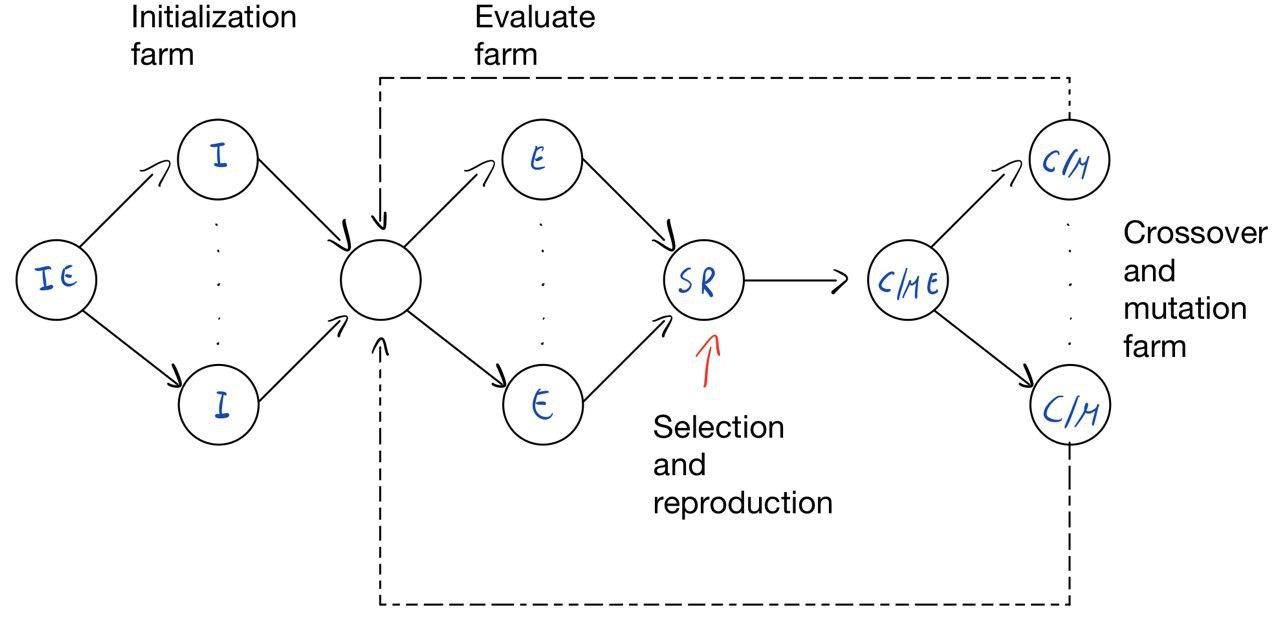
\includegraphics[width=\linewidth]{img/ff_pipeline.jpg}


		\caption{FastFlow pipeline.}
		\label{ff:pipeline}
	\end{figure}
	

	\section{Results}
	The results are shown in graphs, all the execution are made on square matrices. The size tested are 500x500, 1000x1000, 5000x5000 and 1000x1000 with 15 iterations.
	The test are made on Xeon Phi. 
	
	\subsection{Speedup graph}
	\begin{figure}[H]
		\centering
		\begin{minipage}[t]{0.55\linewidth}
			%\includegraphics[width=\linewidth]{BenchMarkGOL/speedup/500/graph500.png}
			%\subcaption{MSE}
		\end{minipage}%
		\begin{minipage}[t]{0.55\linewidth}
			%\includegraphics[width=\linewidth]{BenchMarkGOL/speedup/500/graph500_zoom.png}
			%\subcaption{Accuracy}
		\end{minipage}
		\caption{Speedup curves for 500x500 boards.}
		\label{500}
	\end{figure}

	\begin{figure}[H]
		\centering
		\begin{minipage}[t]{0.55\linewidth}
			%\includegraphics[width=\linewidth]{BenchMarkGOL/speedup/1000/graph1000.png}
			%\subcaption{MSE}
		\end{minipage}%
		\begin{minipage}[t]{0.55\linewidth}
			%\includegraphics[width=\linewidth]{BenchMarkGOL/speedup/1000/graph1000_zoom.png}
			%\subcaption{Accuracy}
		\end{minipage}
		\caption{Speedup curves for 1000x1000 boards.}
		\label{1000}
	\end{figure}

		\begin{figure}[H]
		\centering
		\begin{minipage}[t]{0.55\linewidth}
			%\includegraphics[width=\linewidth]{BenchMarkGOL/speedup/5000/graph5000.png}
			%\subcaption{MSE}
		\end{minipage}%
		\begin{minipage}[t]{0.55\linewidth}
			%\includegraphics[width=\linewidth]{BenchMarkGOL/speedup/5000/graph5000_zoom.png}
			%\subcaption{Accuracy}
		\end{minipage}
		\caption{Speedup curves for 5000x5000 boards.}
		\label{5000}
	\end{figure}

		\begin{figure}[H]
		\centering
		\begin{minipage}[t]{0.55\linewidth}
			%\includegraphics[width=\linewidth]{BenchMarkGOL/speedup/10000/graph10000.png}
			%\subcaption{MSE}
		\end{minipage}%
		\begin{minipage}[t]{0.55\linewidth}
			%\includegraphics[width=\linewidth]{BenchMarkGOL/speedup/10000/graph10000_zoom.png}
			%\subcaption{Accuracy}
		\end{minipage}
		\caption{Speedup curves for 10000x10000 boards.}
		\label{10000}
	\end{figure}

	\subsection{Scalability graph}
		\begin{figure}[H]
		\centering
		\begin{minipage}[t]{0.55\linewidth}
			%\includegraphics[width=\linewidth]{BenchMarkGOL/scalability/500/graph500_scal.png}
			%\subcaption{MSE}
		\end{minipage}%
		\begin{minipage}[t]{0.55\linewidth}
			%\includegraphics[width=\linewidth]{BenchMarkGOL/scalability/500/graph500_scal_zoom.png}
			%\subcaption{Accuracy}
		\end{minipage}
		\caption{Scalability curves for 500x500 boards.}
		\label{500s}
	\end{figure}

	\begin{figure}[H]
		\centering
		\begin{minipage}[t]{0.55\linewidth}
			%\includegraphics[width=\linewidth]{BenchMarkGOL/scalability/1000/graph1000_scal.png}
			%\subcaption{MSE}
		\end{minipage}%
		\begin{minipage}[t]{0.55\linewidth}
			%\includegraphics[width=\linewidth]{BenchMarkGOL/scalability/1000/graph1000_scal_zoom.png}
			%\subcaption{Accuracy}
		\end{minipage}
		\caption{Scalability curves for 1000x1000 boards.}
		\label{1000s}
	\end{figure}

	\begin{figure}[H]
		\centering
		\begin{minipage}[t]{0.55\linewidth}
			%\includegraphics[width=\linewidth]{BenchMarkGOL/scalability/5000/graph5000_scal.png}
			%\subcaption{MSE}
		\end{minipage}%
		\begin{minipage}[t]{0.55\linewidth}
			%\includegraphics[width=\linewidth]{BenchMarkGOL/scalability/5000/graph5000_scal_zoom.png}
			%\subcaption{Accuracy}
		\end{minipage}
		\caption{Scalability curves for 5000x5000 boards.}
		\label{5000s}
	\end{figure}

	\begin{figure}[H]
		\centering
		\begin{minipage}[t]{0.55\linewidth}
			%\includegraphics[width=\linewidth]{BenchMarkGOL/scalability/10000/graph10000_scal.png}
			%\subcaption{MSE}
		\end{minipage}%
		\begin{minipage}[t]{0.55\linewidth}
			%\includegraphics[width=\linewidth]{BenchMarkGOL/scalability/10000/graph10000_scal_zoom.png}
			%\subcaption{Accuracy}
		\end{minipage}
		\caption{Scalability curves for 10000x10000 boards.}
		\label{10000s}
	\end{figure}
\section{Conclusions}
We can see in the graphs that as expected the speedup and the scalability do not increase linearly, but at a certain point reach an inflection point and start decrease or stabilize itself. This can be attribute to the increasing of the overhead of the splitting. In conclusion, it is important to find the right number of parallelism degree and not underestimate the overhead.
\end{document}